\documentclass[11pt]{article}
\usepackage{amsmath,amsthm,amssymb,fullpage,graphicx,hyperref,listings}
\usepackage{listings,color,setspace}
\author{Andy Reagan}
\title{Math 337 Homework 16}

     \def\NN{\mathbb{N} }
     \def\ZZ{\mathbb{Z} }
     \def\QQ{\mathbb{Q} }
     \def\RR{\mathbb{R} }
     \def\CC{\mathbb{C} }
     \def\f{\frac }
     \def\b{\begin }
     \def\e{\end }
     \def\Log{\text{Log} \,}
     \def\Re{\text{Re} \, }
     \newcommand{\pdiff}[2]{\frac{\partial #1}{\partial #2}}
     \newcommand{\partialdiff}[2]{\frac{\partial #1}{\partial #2}}
     \newcommand{\pdiffsq}[2]{\frac{\partial^2 #1}{{\partial #2}^2}}
     \newcommand{\pdiffcu}[2]{\frac{\partial^3 #1}{{\partial #2}^3}}
     \newcommand{\pdiffhi}[3]{\frac{\partial^#3 #1}{{\partial #2}^#3}}
     \newcommand{\diff}[2]{\frac{{\rm d}#1}{{\rm d}#2}}
     \newcommand{\diffsq}[2]{\frac{{\rm d}^{2}#1}{{\rm d} {#2}^2}}
     \newcommand{\diffhi}[3]{\frac{{\rm d}^#3 #1}{{\rm d} {#2}^#3}}
     \newcommand{\tdiff}[2]{\mbox{d} #1/\mbox{d} #2}
     \newcommand{\tdiffsq}[2]{\mbox{d}^{2} #1/\mbox{d} {#2}^2}
     \newcommand{\tpdiff}[2]{\partial #1/\partial #2}
     \newcommand{\tpdiffsq}[2]{\partial^2 #1/\partial {#2}^2}
     \newcommand{\bvec}[1]{\vec{ {\bf #1 } }}
     \newcommand{\oh}[1]{O(h^{{#1}})}

\lstset{language=MATLAB,
basicstyle=\ttfamily\scriptsize\singlespacing,
keywordstyle=\color{black},
stringstyle=\color{black},
commentstyle=\color{black},
morecomment=[l][\color{black}]{\#},
frame=L,
xleftmargin=\parindent,
%%numbers=left,                   %% where to put the line-numbers
%%numberstyle=\scriptsize,      %% the size of the fonts that are used for the line-numbers
%%stepnumber=1,                   %% the step between two line-numbers. If it is 1 each line will be numbered
numbersep=5pt,
breaklines=true,        %% sets automatic line breaking
breakatwhitespace=false,    %% sets if automatic breaks should only happen at whitespace
escapeinside={\%*}{*)} 
}

%% example code insert
%% \lstinputlisting[language=Matlab]{andy_hw12_prb01.m}

%% example figure
%% \begin{figure}[h!]
%%   \centering
%%     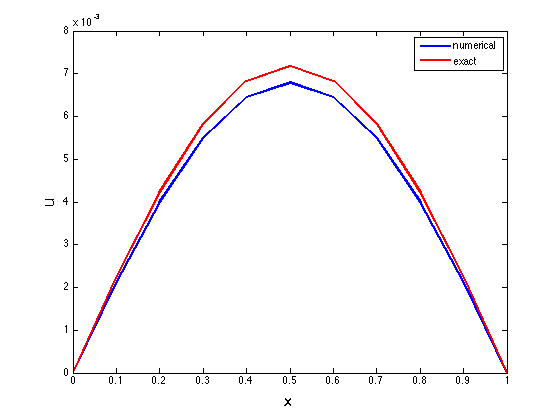
\includegraphics[width=0.45\textwidth]{andy_hw12_prb01_02.png}
%%   \caption{The numerical and exact solution for $h=0.1$.}
%% \end{figure}

%% start problem on next page
%% \clearpage
%% \pagebreak

\begin{document}
\maketitle

\begin{enumerate}

\item I stick with MATLAB for this one, and the following code produces a plot with 6 stages of the evolution of the solution.
I'll note that MATLAB's \verb|quad| fails to properly integrate the piecewise function, so I use \verb|integral| with the option \verb|ArrayValued| set to \verb|true|.

Since the solution is supported at any $x$ that overlaps $[0,2]$ at time $t$, we have the solution is always supported by $[0,2]$.
The solution is support $ct$ to the right of $2$, since the lower integration bound $(x-ct)$ will overlap, and similarly supported $ct$ to the left of 0.
Therefore, the width of the support is $2ct+2$.

\lstinputlisting[language=Matlab]{andy_hw16_prb01.m}

\begin{figure}[h!]
  \centering
    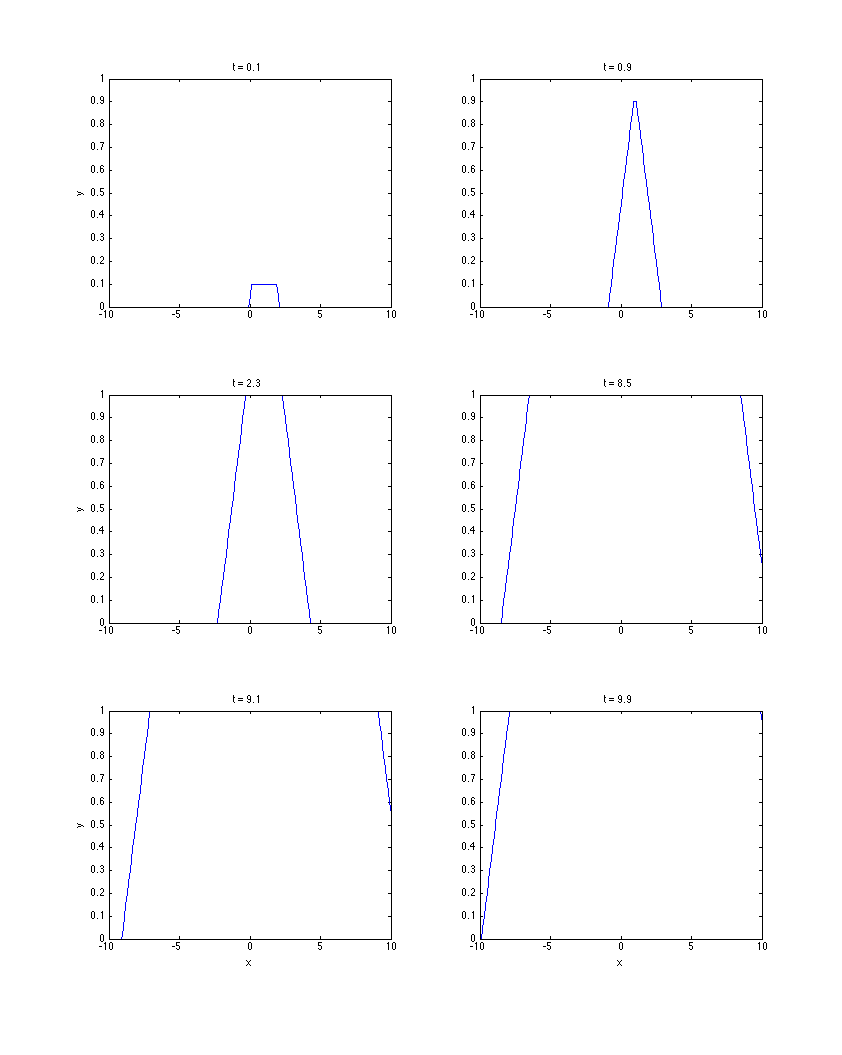
\includegraphics[width=1.05\textwidth]{andy_hw16_prb01_03.png}
   \caption{Six panels of evolution of the D'Alembert solution.
   I observe three qualitatively different profiles.
   Namely, in the first phase, the height and support of the solution are both growing.
   When the height has reached 1, the solution attains a peak.
   And when $t>1$, the solution remains with a plateau at $1$, and grows in width.
   My code (above) plots the time evolution.}
\end{figure}

\clearpage
\pagebreak
\item Plugging 16.7 into 16.6 we have the two equations:
\[ F(x) + G(x) = \phi (x) ~~~~~~~~~ -cF_x(x) + cG_x(x) = \psi (x) .\]
Differentiating the first equation wrt $x$, these equations become
\[ F_x(x) + G_x(x) = \phi _x(x) ~~~~~~~~~ -cF_x(x) + cG_x(x) = \psi (x) .\]
Solving the first for $F$, and plugging into the second, we have:
\begin{align*} -c\left ( \phi _x(x) - G_x(x) \right )  + cG_x(x) = \psi (x) \\
-\phi _x(x) + G_x(x)  + G_x(x) = \f{1}{c}\psi (x) \\
G_x(x) = \f{1}{2c}\psi (x) + \f{1}{2} \phi _x (x)\\
G(x) = \f{1}{2c}\int _{-\infty} ^{x} \psi (s) ds + \f{1}{2} \phi (x)\end{align*}
where in the last step we have integrated from $-\infty$ to $x$, applied the Fundamental Theorem of Calculus, and rely upon the assumption that there no disturbance coming in from $x= -\infty$, such that $G(-\infty) = \phi(-\infty) = 0$.

Similarly, we can solve for $F$:
\begin{align*} c\left ( \phi _x(x) - F_x(x) \right )  - cF_x(x) = \psi (x) \\
\phi _x(x) - F_x(x)  - F_x(x) = \f{1}{c}\psi (x) \\
F_x(x) = -\f{1}{2c}\psi (x) + \f{1}{2} \phi _x (x)\\
F(x) = -\f{1}{2c}\int _{-\infty} ^{x} \psi (s) ds + \f{1}{2} \phi (x)\end{align*}


This verifies Eq (16.28a).
Simply evaluating $G$ and $F$ at $(x\pm ct)$ , respectively, we have:
\begin{align*} F(x-ct) = -\f{1}{2c}\int _{-\infty} ^{x-ct} \psi (s) ds + \f{1}{2} \phi (x-ct)~~~~~~~~~~G(x+ct) = \f{1}{2c}\int _{-\infty} ^{x+ct} \psi (s) ds + \f{1}{2} \phi (x+ct)\end{align*}
which verifies Eq (16.28b).

Finally, we plug the above (16.28b) into Eq (16.6) and we have
\begin{align*} u(x,t) &= -\f{1}{2c}\int _{-\infty} ^{x-ct} \psi (s) ds + \f{1}{2} \phi (x-ct) +  \f{1}{2c}\int _{-\infty} ^{x+ct} \psi (s) ds + \f{1}{2} \phi (x+ct)\\
&= \f{1}{2} \left ( \phi (x-ct)  + \phi (x+ct) \right ) +  \f{1}{2c}\int _{x-ct} ^{x+ct} \psi (s) ds\end{align*}
where we have cancelled the overlapping portions of the integral (formally, splitting the integral to $x+ct$ into the overlapping and non-overlapping parts, then cancelling).
This verifies Eq (16.8).
\end{enumerate}
\end{document}



